\section{Firmware}
\subsection{uC/OS-III - Distribución de tareas}
Para el control del sistema utilizaremos el sistema operativo en tiempo real
\uCOS . En este sistema tendremos dos tareas principales (además de las
del sistema operativo), una se encargará de controlar las tiras de LEDs y la
otra de la comunicación por infrarrojos.

\begin{figure}[!ht]
	\centering

	\includegraphics[width=\textwidth]{images/tareas}

	\caption{Diagrama de tareas}
	\label{fig:tareas}
\end{figure}

\subsection{Control de Tira de LEDs}
La tarea que controla las tiras de LEDs es crítica, por lo que es la más
prioritaria. Ésta puede recibir dos tipos de mensajes, uno enviado desde la
interrupción del ``\textsl{Input Capture}'' que envía el número de ticks
transcurridos desde la última vuelta. El otro es un mensaje en blanco,
simplemente para indicar que se han de actualizar las tiras de LEDs.

Una vez que la tarea recibe el número de ticks, calcula el periodo de rotación
de la rueda, cada cuánto se tienen que actualizar las tiras y configura el timer
en consecuencia, para que éste le envíe un mensaje cuando toque actualizarlas.

\subsubsection{Control de los LEDs}
\paragraph{Las tiras de LEDs} disponen de una entrada de datos y un protocolo
propio de transmisión de datos. Los LEDs utilizan 3x8 bits en formato GRB para
establecer su color. Estos datos se le transmiten en serie de forma asincrona.
Cada LEDs almacena sus 24bits y luego retransmite lo que recibe a los
siguientes. Una vez que todos los LEDs tienen sus datos, se ha de transmitir una
señal de 50$\mu s$ a cero para que actualicen sus PWMs y cambien el color. Para
generar la forma de onda que esperan las tiras usamos un puerto SPI con una
configuración adecuada.

\paragraph{Las imágenes} las cambiamos de formato con el programa
``MatrixAngle'' (ver \refcont{sec:matrixAngle}), de forma que almacenamos el
color de cada led de cada tira para cada instante de activación (al que llamamos
\textbf{radio}). Luego las guardamos en la memoria FLASH al cargar el programa.

Cada vez que se han de actualizar los LEDs la tarea hace lo siguiente:

\begin{enumerate}
	\item Lee el color de los LEDs para la posición actual de cada tira
		(radio).
	\item Se genera el buffer que se enviara por el puerto SPI para generar
		la señal en el formato que esperan las tiras.
	\item Se activa el DMA para que envíe este buffer por el puerto SPI.
	\item Se incrementa el radio para la siguiente iteración, o se cambia la
		imagen si ya se ha dibujado la actual.
\end{enumerate}

\subsection{Tarea de comunicación}
Cuando el USART recibe un dato por infrarrojos se activa la rutina de
interrupción encargada de reconocer una trama y enviársela a la tarea de
comunicación. Como en \uCOS\ los mensajes solo guardan un puntero a los datos,
necesitamos reservar memoria para cada nueva trama reconocida. Para esto
utilizamos la funcionalidad que nos proporciona \uCOS\ para asignar y desasignar
secciones de memoria. La rutina de interrupción reserva memoria para la trama
que está reconociendo (si no la ha reservado ya) y la tarea de comunicación la
libera una vez que ha terminado de procesarla.

\newpage
\subsubsection{Sincronismo de trama}
Para identificar y sincronizar las tramas utilizamos el método de ``principio y
cuenta'' con carácter delimitador y CRC. El formato de la trama lo podemos
apreciar en la figura \reffig{fig:frame-sinc}, e iremos explicando cada campo a
continuación.

\begin{figure}[!ht]
	\centering
	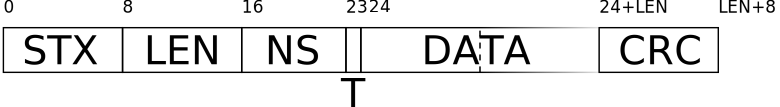
\includegraphics[width=\textwidth]{images/frame-sinc}
	\caption{Formato de la trama para el sincronismo}
	\label{fig:frame-sinc}
\end{figure}

\begin{itemize}
	\item \textbf{STX}: Carácter especial que indica el comienzo de la
		trama.
	\item \textbf{LEN}: Longitud del campo de datos.
	\item \textbf{NS y T}:  Con objeto de ampliar la comunicación a
		\textsl{half-duplex} con \textsl{ACK} y \textsl{retroceder-N},
		también introducimos en la trama un 7 bits para el número de
		secuencia y un bit para ceder la comunicación.
	\item \textbf{DATA}: Datos a transmitir.
	\item \textbf{CRC}: CRC-8 de la trama completa.
	\item \textbf{DLE}: Carácter de escape que desactivará la interpretación
		como carácter especial del siguiente byte recibido. Sirve para
		poder transmitir bytes iguales que STX sin que se reinicie el
		reconocimiento de la trama.
\end{itemize}

Para realizar el sincronismo de tramas hemos implementado una pequeña máquina de
estados, que se muestra en la figura \reffig{fig:stateMachine-sinc}. El escape de
caracteres se ha implementado desactivando el reconocimiento en la máquina de
estados, no como estados a parte.

\begin{figure}[!ht]
	\centering
	\includegraphics[width=\textwidth]{images/stateMachine-sinc}
	\caption{Máquina de estados para el sincronismo de tramas}
	\label{fig:stateMachine-sinc}
\end{figure}

\subsubsection{Formato de tramas datos y comandos}
Por el momento solo está implementado el reconocimiento de comandos para cambiar
la imagen y la animación a mostrar. El formato de trama que utilizamos es el que
se muestra en la figura \reffig{fig:frame-data}.

\begin{figure}[!ht]
	\centering
	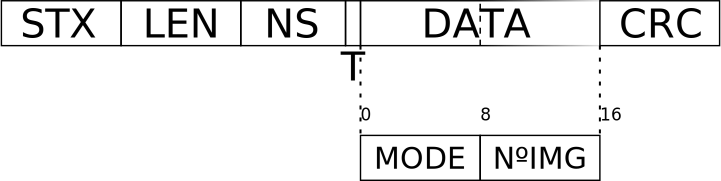
\includegraphics[width=\textwidth]{images/frame-data}
	\caption{Trama para el envío de comandos}
	\label{fig:frame-data}
\end{figure}

\newpage
\begin{itemize}
	\item \textbf{MODE}: Indica si se quiere poner el sistema en modo
		animación cíclica o que se quiere mostrar una imagen u animación
		específica.
	\item \textbf{N\_ANIM}: Indica el índice de la imagen u animación que se
		quiere mostrar.
\end{itemize}
